\documentclass[numbers=noenddot,12pt,a4paper]{scrartcl}
\usepackage[greek,ngerman]{babel}
\usepackage[T1]{fontenc}
\usepackage[utf8]{inputenc}
\usepackage{fullpage}
\usepackage{libertine}
\usepackage{ziffer}
\usepackage{graphicx}
\usepackage{units}
\usepackage[infoshow]{tabularx}
\usepackage{amsmath}
\usepackage{amssymb}
\usepackage{wrapfig}
\usepackage{esint}
\usepackage{float}
\usepackage{wrapfig}
\usepackage[font=small]{caption}
\usepackage{subcaption}
\usepackage{lscape}
\usepackage{hyperref}

\renewcommand{\thefigure}{Abb. \arabic{figure}}

\captionsetup[wrapfigure]{name=}
\captionsetup[figure]{name=}
\newcommand{\degree}{^\circ}
\newcommand{\diff}{\textnormal{d}}
\newcommand{\tenpo}[1]{\cdot 10^{#1}}
\newcommand{\greek}[1]{\greektext#1\latintext}
\newcommand{\ix}[1]{_\text{#1}}
\newcommand{\imag}{\mathbf{i}}
\newcommand{\tilt}[1]{\textit{#1}}
\newcommand{\grad}[1]{\textit{grad}\left(#1\right)}
\newcommand{\divergenz}[1]{\textit{div}\left(#1\right)}
\newcommand{\euler}{\mathnormal{e}}
\newcommand{\fett}[1]{\textbf{#1}}
\newcommand{\partiell}[2]{\frac{\partial #1}{\partial #2}}
\newcommand{\partiellz}[2]{\frac{\partial^2 #1}{\partial #2^2}}
\newcommand{\partielld}[2]{\frac{\partial^3 #1}{\partial #2^3}}

\title{Protokoll: Akustische Experimente zur Modellierung von Quanten-Phänomenen}
\author{Tom Kranz, Philipp Hacker}
\date{\today}

\begin{document}
\maketitle
\begin{center}
Betreuer: S. Peglow\\
Versuchsdatum: 11.11.2014\\
\begin{table}[h]
\centering
Note: %TODO Gute Note erhalten :)
\begin{tabularx}{1.5cm}{|X|}
\hline \\ \\
\hline
\end{tabularx}
\end{table}
\end{center}
\vspace*{\fill}
\tableofcontents
\vfill
\newpage
\section{Einleitung}
In diesem Versuch sollen die Eigenschaften grundlegender quantenmechanischer Systeme anhand einfacher Experimente mit Schall veranschaulicht werden. Dazu werden Ähnlichkeiten der quantenmechanischen Bewegungsgleichung, der Schrödinger-Gleichung, und der Bewegungsgleichung für klassische Wellenerscheinungen, der Wellengleichung, unter bestimmten Randbedingungen ausgenutzt, aber auch auf die Unterschiede aufmerksam gemacht.\\
Die durchgeführten Experimente modellieren ein Teilchen im Kastenpotential, ein Elektron im Coulomb-Feld eines Atomkerns, sowohl ungestört, als auch unter Einwirkung eines symmetriebrechenden äußeren Feldes und ein Elektron im $\text{H}_2^+$-Molekül bei unterschiedlich starker Kopplung.
\section{Grundlagen}
In der Quantenmechanik werden Zustände durch sogenannte Wellenfunktionen beschrieben. Sie sind Lösungen der Schrödinger-Gleichung für die Randbedingungen, denen das betrachtete physikalische Objekt unterliegt. In Ortsdarstellung hat sie im Allgemeinen die Form:
\begin{align}
\imag\hbar\frac{\partial\psi}{\partial t}=-\frac{\hbar^2}{2m}\vec{\nabla}^2 \psi+V(\vec{r})\psi\label{eq:schro}
\end{align}
Mit der Wellenfunktion $\psi(\vec{r},t)$, dem reduzierten Planckschen Wirkungsquantum $\hbar$, der Teilchenmasse $m$, dem Laplace-Operator $\vec{\nabla}^2=\overset{3}{\underset{i=1}{\sum}}\frac{\partial^2}{\partial r_i^2}$ und dem ortsabhängigen Potential $V(\vec{r})$.\\
Die klassische Wellengleichung hat im Allgemeinen die Form:
\begin{align}
\frac{1}{c^2}\frac{\partial^2 u}{\partial t^2}=\vec{\nabla}^2 u
\end{align}
Hier ist $u(\vec{r},t)$ eine physikalische Größe (zum Beispiel der Druck $p$) und $c$ die Ausbreitungsgeschwindigkeit der Welle.\\
Sofort fällt die Ähnlichkeit zwischen den beiden Gleichungen auf: Die linke Seite ist eine Ableitung nach der Zeit, die rechte enthält einen Orts-Differentialoperator. Jedoch ist die Zeitableitung in der Wellengleichung eine zweifache, in der Schrödinger-Gleichung eine einfache, aber mit der imaginären Einheit als Vorfaktor. Auch tritt in der Wellengleichung kein Potential auf.
\subsection{Das Teilchen im Kastenpotential}
Das Teilchen im Kastenpotential ist ein Modell eines Teilchens, das sich in einem schwachen Potential bewegt, das abrupt von hohen Potentialwänden umgeben ist. Das (eindimensionale) Modell vereinfacht dies auf das Potential
\begin{align}
V(x)=\left\{\begin{array}{ll}
0&,\,0< x< L \\ 
\infty &\text{, ansonsten}
\end{array} \right.
\end{align}
Wobei $L$ die Länge des Kastens darstellt. Außerhalb des Kastens können keine Zustände existieren, weswegen dort die Wellenfunktion $\psi=0$ ist; innerhalb des Kastens vereinfacht sich die Schrödingergleichung zu
\begin{align}
\imag\hbar\frac{\partial\psi}{\partial t}=-\frac{\hbar^2}{2m}\frac{\partial^2\psi}{\partial x^2}
\end{align}
Diese wird durch eine Linearkombination von Eigenzuständen der stationären Schrödingergleichung, multipliziert mit einem Phasenfaktor $\exp\left(-\imag\omega t\right)$, gelöst. Die stationäre Schrödingergleichung ist die Eigenwertgleichung der rechten Seite der Gleichung (\ref{eq:schro}), in diesem Falle:
\begin{align}
E\psi=-\frac{\hbar^2}{2m}\frac{\partial^2\psi}{\partial x^2}\label{eq:kasten}
\end{align}
Die Lösungen dieser Gleichung sind, unter Beachtung der Randbedingungen, Sinus-Funktionen
\begin{align}
\psi(x)=A\sin\left(kx\right)\text{ mit }k=n\frac{\pi}{L};\;n\in\mathbb{N}\label{eq:kastenl}
\end{align}
Über die aus Gleichung (\ref{eq:kasten}) folgende Dispersionsrelation $E=\frac{\hbar^2k^2}{2m}$ bewirken die Randbedingungen auch eine Quantelung der Energie der Eigenzustände.
\subsubsection{Analogon: Stehende Schallwellen in der Röhre}
Werden Schallwellen in einem Rohr angeregt, werden sie von den Enden des Rohres reflektiert und alle im Rohr befindlichen Wellen überlagern sich -- stehende Wellen entstehen. Wenn sich alle im Rohr befindlichen Schallwellen konstruktiv überlagern, spricht man von Resonanz. Für die konstruktive Überlagerung von einfallender und reflektierter Welle muss die Wellenlänge $\lambda$ der Schallwelle ein halbzahliges Vielfaches der Rohrlänge $L$ sein:
\begin{align}
\frac{n}{2}\lambda=L
\end{align}
Schaut man zurück auf Gleichung (\ref{eq:kastenl}), fällt auf, dass bei Identifizierung von $k=\frac{2\pi}{\lambda}$ genau der gleiche Ausdruck entsteht. Resonanzen von Schallwellen in einem Rohr lassen sich also als einfache Modellierung der Eigenfunktionen des Teilchens im Kasten ansehen. Allerdings findet hier die Energie, mit ihrer quadratischen Abhängigkeit von der Quantenzahl $n$ keine Entsprechung. Auch sollte beachtet werden, dass die quantenmechanische Wellenfunktion ihre Knotenpunkte an den Rändern hat, während der Druck bei der Resonanz, bedingt durch die Position der Quelle der Erregung, Wellenberge an den Rändern aufweist.
\subsection{Das Wasserstoffatom}
Das Wasserstoffatom ist das einfachste Atom; es besteht lediglich aus einem Proton und einem Elektron. Bei diesem Problem tritt das Coulomb-Potential $V(\vec{r})=V(r)=\frac{-e^2}{4\pi\varepsilon_0 r}$ auf, die stationäre Schrödinger-Gleichung für die Wellenfunktion des Elektrons lautet daher:
\begin{align}
E\psi=-\frac{\hbar^2}{2m}\vec{\nabla}^2 \psi-\frac{e^2}{4\pi\varepsilon_0 r}\psi\label{eq:wass}
\end{align}
Schreibt man diese in Kugelkoordinaten um:
\begin{align}
E\psi=\frac{\hbar^2}{2mr^2}\partiell{}{r}\left(r^2\partiell{\psi}{r}\right)+\frac{\hbar^2}{2mr^2\sin(\theta)}\partiell{}{\theta}\left(\sin(\theta)\partiell{\psi}{\theta}\right)+\frac{\hbar^2}{2mr^2\sin^2(\theta)}\partiellz{\psi}{\varphi}-\frac{e^2}{4\pi\varepsilon_0 r}\psi,\label{eq:wassku}
\end{align}
so eröffnet sich ein Separationsansatz: $\psi(r,\theta,\varphi)=Y^m_l(\theta,\varphi)\chi_l(r)$. Hierbei sind die Kugelflächenfunktionen $Y_l^m$ die Lösungen des Winkelanteils von Gleichung (\ref{eq:wassku}):
\begin{align}
-\frac{1}{\sin(\theta)}\partiell{}{\theta}\left(\sin(\theta)\partiell{Y_l^m}{\theta}\right)-\frac{1}{\sin^2(\theta)}\partiellz{Y_l^m}{\varphi}=l(l+1)Y_l^m
\end{align}
und $\chi_l(r)$ die Lösungen des radialen Anteils von Gleichung (\ref{eq:wassku}):
\begin{align}
-\frac{\hbar^2}{2mr}\partiellz{}{r}\left(r\chi_l\right)-\frac{l(l+1)\hbar^2}{2mr^2}\chi_l--\frac{e^2}{4\pi\varepsilon_0 r}\chi_l=E\chi_l
\end{align}
\subsubsection{Analogon: sphärischer akustischer Resonator}\label{ch:sph}
Werden Schallwellen in einer Hohlkugel angeregt, folgt der Druck innerhalb der Kugel der Wellengleichung
\begin{align}
\partiellz{p}{t}=\frac{1}{\rho\kappa}\vec{\nabla}^2p
\end{align}
Hier sind $\rho$ die Luftdichte und $\kappa$ die Kompressibilität. Ähnlich, wie die stationäre Schrödingergleichung auf einem Separationsansatz beruht, lässt sich diese Gleichung durch den Ansatz $p(\vec{r},t)=p(\vec{r})\cos(\omega t)$ in eine stationäre Gleichung, die Helmholtzgleichung, überführen:
\begin{align}
\omega^2p(\vec{r})=-\frac{1}{\rho\kappa}\vec{\nabla}^2p(\vec{r})\;\text{ bzw. }\;-\frac{\omega^2}{c^2}p=\vec{\nabla}^2p
\end{align}
Wie Gleichung (\ref{eq:wassku}) bringt auch hier das Umschreiben in Kugelkoordinaten die Möglichkeit der Separation $p(r,\theta,\varphi)=Y_l^m(\theta,\varphi)f(r)$ mit sich:
\begin{align}
-\frac{1}{r^2}\partiell{}{r}\left(r^2\partiell{p}{r}\right)-\frac{1}{r^2\sin(\theta)}\partiell{}{\theta}\left(\sin(\theta)\partiell{p}{\theta}\right)-\frac{1}{r^2\sin^2(\theta)}\partiellz{p}{\varphi}=\frac{\omega^2}{c^2}p\label{eq:sph}
\end{align}
Der Winkelanteil der Gleichung ist:
\begin{align}
-\frac{1}{\sin(\theta)}\partiell{}{\theta}\left(\sin(\theta)\partiell{Y_l^m}{\theta}\right)-\frac{1}{\sin^2(\theta)}\partiellz{Y_l^m}{\varphi}=l(l+1)Y_l^m,
\end{align}
wohingegen der radiale Anteil wie folgt aussieht:
\begin{align}
-\partiellz{f}{r}-\frac{2}{r}\partiell{f}{r}+\frac{l(l+1)}{r^2}f(r)=\frac{\omega^2}{c^2}f(r)
\end{align}
Sofort fällt auf, dass die Winkelanteile der Gleichungen (\ref{eq:wassku}) und (\ref{eq:sph}) und damit auch der Wellenfunktion, beziehungsweise der Funktion des Drucks, identisch sind. Man kann also mit Schallwellen in einer Hohlkugel die Winkelabhängigkeit der Wellenfunktion des Elektrons im Wasserstoffatom modellieren. Die Unterschiede in den Radialanteilen lassen jedoch keine Analogie zwischen den radialen Abhängigkeiten der Wellenfunktion und des Drucks zu.
\subsubsection{Gebrochene Symmetrie}
Der sphärische Resonator in unserem Versuch besteht aus zwei halben Hohlkugeln, die zusammengesteckt werden, um eine volle Hohlkugel zu bilden. In die obere Hälfte ist ein Mikrofon integriert, in die untere ein Lautsprecher (und ein Mikrofon; dieses wird jedoch nicht genutzt) und beide haben zur Kontaktebene einen Winkel von $\unit[45]{\degree}$. Bei einer perfekten Kugel wird die Symmetrieachse (die $z$-Achse) durch die Position des Lautsprechers bestimmt, weswegen nur diejenigen Resonanzen angeregt werden können, deren Kugelflächenfunktionen bei $\theta=0$ nicht verschwinden. Dies kann durch Erzwingen einer Symmetrieachse, zum Beispiel durch Streckung der Kugel, geändert werden -- die Symmetrieachse ist nun senkrecht zur Kontaktebene und der Lautsprecher kann auch Resonanzen anregen, deren Amplituden auf der Symmetrieachse verschwinden.
\subsection{Das $\text{H}_2^+$-Molekül}
Koppelt man zwei sphärische Resonatoren über eine Lochblende miteinander, simuliert man die Überlagerung zweier Systeme, wie sie in \ref{ch:sph} beschrieben sind. Dies kommt in der Natur bei der Bildung von Molekülen vor: Die Kerne der einzelnen Atome bilden zusammen ein Potential aus, das die Wellenfunktionen der Elektronen bestimmt. Beim $\text{H}_2^+$-Molekül sind dies zwei Wasserstoffkerne und da sich nur ein einziges Elektron in diesem System befinden, treten keine Störungen durch Elektron-Elektron-Wechselwirkungen auf und die Überlagerung zweier Wasserstoff-Systeme stelt eine gute Näherung für die Verhältnisse im Molekül dar. Für die Lochblende können hierbei verschiedene Größen gewählt werden, was in der Molekül-Beschreibung einer größeren Kopplung der Systeme, also einem geringeren Kernabstand entspricht.
\section{Durchführung}
\subsection{Röhrenresonanz}
Zuerst wurde ein Röhrenresonator mittels eines Lautsprechers und eines Mikrofons auf seine Resonanzen untersucht. Der Lautsprecher wurde mit variabler Frequenz betrieben und das Mikrofon-Signal von einem Oszilloskop aufgenommen -- Resonanzen äußerten sich durch Maxima im Ausgangssignal. Die gefundenen Resonanzfreuqenzen wurden für verschiedene Resonatorlängen in \ref{img:resonatorhand} aufgetragen und an lineare Funktionen mittels Methode der kleinsten Quadrate angepasst. Bei kürzeren Resonatoren wurde dabei eine scheinbare Resonanz bei ungefähr $\unit[420]{Hz}$ gefunden, die aber, vor allem vor dem Hintergrund der Theorie, nicht zu den restlichen Werten passt und von uns daher als Fehlmessung eingestuft wurde. Ansonsten wurden die Messwerte exakt von der Theorie vorausgesagt, was sich in den guten linearen Fits widerspiegelt.
\begin{figure}[H]
	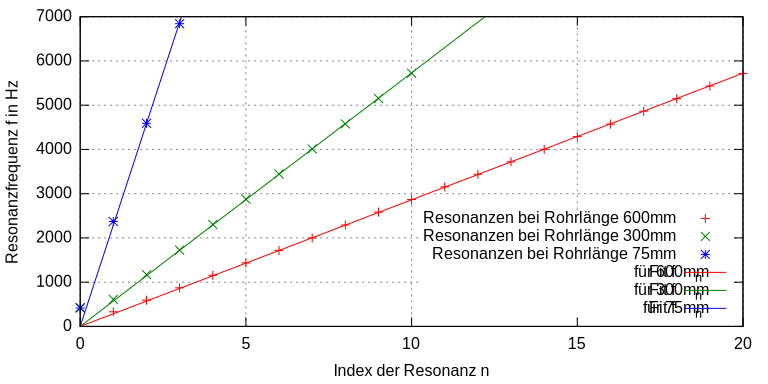
\includegraphics[width=\textwidth]{messwerte/resonanzfrequenzen.pdf}
	\caption{Resonanzfrequenzen der Röhre bei verschiedenen Längen}\label{img:resonatorhand}
\end{figure}
Dann wurden von der Soundkarte eines Computers verschiedene Frequenzen erzeugt und zugleich die Intensitäten über das Mikrofon gemessen. Die Variation der Frequenz erfolgte in $\unit[10]{Hz}$-Schritten und die Messung bestätigt das bereits von Hand bestimmte Resonanzfrequenzspektrum in einer etwas größeren Umgebung. Zum Vergleich wurden in \ref{img:resonatorcomp} auch die Resonanzfrequenzen aus \ref{img:resonatorhand} gekennzeichnet. Wieder zeigt sich die gute Übereinstimmung des Experiments mit der Theorie, da die Intensitätsmaxima stets den gleichen Abstand voneinander aufweisen.
\begin{figure}[H]
	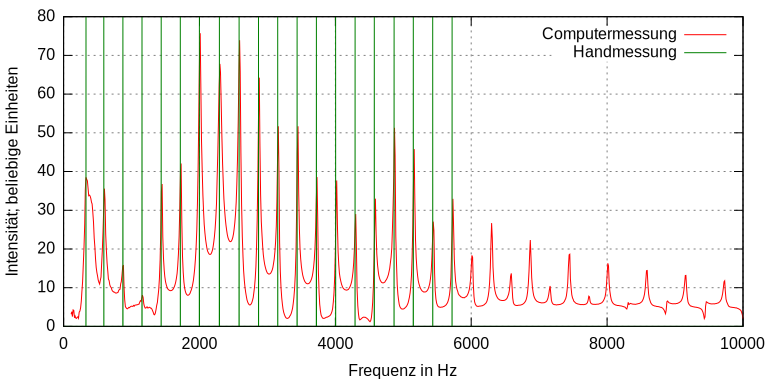
\includegraphics[width=\textwidth]{messwerte/resonanzfrequenzencomputer.pdf}
	\caption{Vom Computer gefundende Resonanzen der Röhre bei $L=\unit[600]{mm}$}\label{img:resonatorcomp}
\end{figure}
\subsection{Sphärischer Resonator}
\begin{figure}[H]
	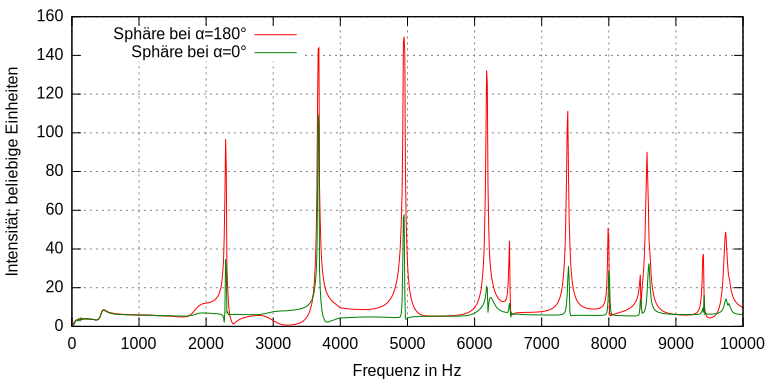
\includegraphics[width=\textwidth]{messwerte/sphaeren0-10kHz.pdf}
	\caption{Übersichtsspektren für sphärischen Resonator}\label{img:ubersicht}
\end{figure}
Beim sphärischen Resonator wurde ähnlich verfahren wie bei der computergestützten Vermessung der Resonanzfrequenzspektren der Röhren. Das Mikrofon konnte gegen den Lautsprecher verschoben werden, sodass ihre "`Achsen"' einen Winkel zwischen $0$ ($\alpha=\unit[180]{\degree}$) und $\unit[90]{\degree}$ ($\alpha=\unit[0]{\degree}$) zueinander einnehmen konnten. \ref{img:ubersicht} zeigt das Ergebnis des Durchlaufs des Frequenzspektrums von $\unit[0]{Hz}$ bis $\unit[10]{kHz}$ in $\unit[10]{Hz}$-Schritten. Die Resonanzen sind hier deutlich an den Intensitätsmaxima zu erkennen; sie können unabhängig von der Mikrofonstellung festgestellt werden. In \ref{img:detail} wurde ein engerer Bereich ($\unit[4,85]{kHz}-\unit[5]{kHz}$) mit einer kleineren Schrittweite ($\unit[0,2]{Hz}$) und zusätzlichen Mikrofonstellungen vermessen. Es zeigt sich, dass das Maximum kurz vor $\unit[5]{kHz}$ eigentlich zwei Maxima beinhaltet, deren Positionen aber nicht von der Mikrofonstellung abhängen, ihre Intensitäten aber schon. Dies ist Grundlage für die \ref{img:l1}, \ref{img:l2} und \ref{img:l3}: Hier wurden die Intensitäten unter verschiedenen Mikrofonstellungen gemessen und über den Winkel zwischen Lautsprecher- und Mikrofonachse $\theta=\arccos\left(\frac{1}{2}\cos\left(\alpha\right)-\frac{1}{2}\right)$ in einer polaren Darstellung mit $r\propto I$ aufgetragen. Die senkrechte Linie bezeichnet dabei die Mikrofonachse ($\theta=0$). Zum Vergleich mit der Theorie sind in den \ref{img:l1y}, \ref{img:l2y} und \ref{img:l3y} die entsprechenden Kugelflächenfunktionen abgebildet. Es lässt sich daraus schließen, dass die $l=1;m=0$-, $l=2;m=0$- und $l=3;m=0$-Zustände jeweils von den Frequenzen $\unit[2300]{Hz}$, $\unit[3700]{Hz}$ und $\unit[4925]{Hz}$ angeregt werden.
\begin{figure}[H]
	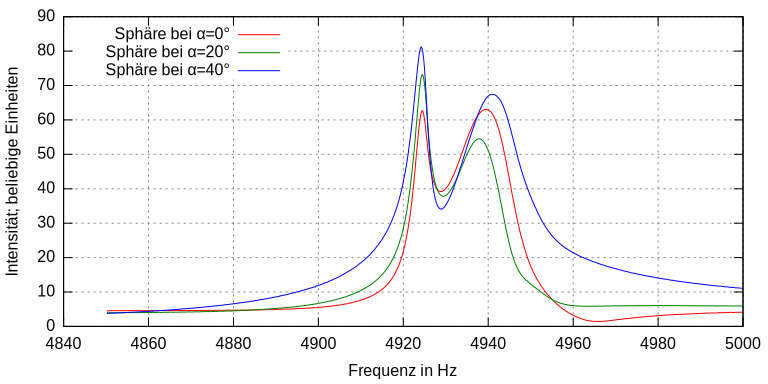
\includegraphics[width=\textwidth]{messwerte/sphaerendetailiertesspektrum.pdf}
	\caption{Detaillierte Spektren nahe $\unit[5]{kHz}$ für verschiedene Mikrofonpositionen}\label{img:detail}
\end{figure}
\begin{figure}[H]
\centering
	\begin{subfigure}[h]{0.3\textwidth}
	\begin{subfigure}[b]{\textwidth}
		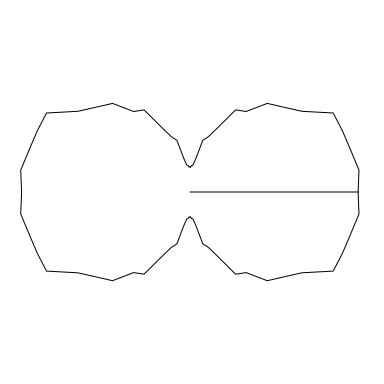
\includegraphics[angle=90,origin=c,width=\textwidth]{messwerte/polarl1.pdf}
		\caption{gemessen bei $\unit[2300]{Hz}$} \label{img:l1}
	\end{subfigure}
	\begin{subfigure}[b]{\textwidth}
		\includegraphics[width=\textwidth]{Spherical_Harmonics_deg3l1m0.png}
		\caption{$Y_l^m$ mit $l=1;m=0$} \label{img:l1y}
	\end{subfigure}
	\end{subfigure}
	\begin{subfigure}[h]{0.3\textwidth}
	\begin{subfigure}[b]{\textwidth}
		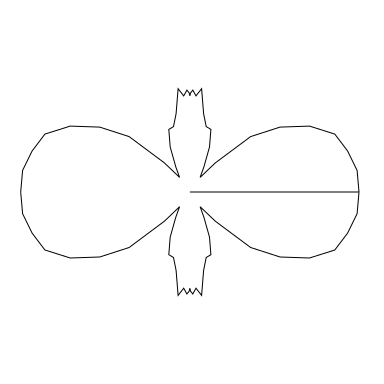
\includegraphics[angle=90,origin=c,width=\textwidth]{messwerte/polarl2.pdf}
		\caption{gemessen bei $\unit[3700]{Hz}$} \label{img:l2}
		\end{subfigure}
		\begin{subfigure}[b]{\textwidth}
			\includegraphics[width=\textwidth]{Spherical_Harmonics_deg3l2m0.png}
			\caption{$Y_l^m$ mit $l=2;m=0$} \label{img:l2y}
			\end{subfigure}
		\end{subfigure}
			\begin{subfigure}[h]{0.3\textwidth}
	\begin{subfigure}[b]{\textwidth}
		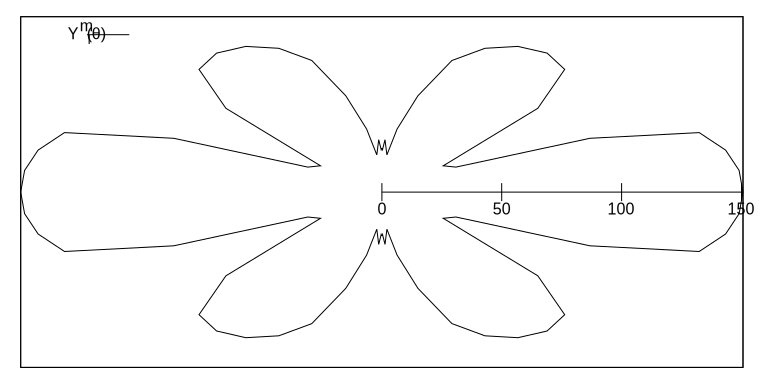
\includegraphics[angle=90,origin=c,width=\textwidth]{messwerte/polarl3.pdf}
		\caption{gemessen bei $\unit[4925]{Hz}$} \label{img:l3}
		\end{subfigure}
		\begin{subfigure}[b]{\textwidth}
			\includegraphics[width=\textwidth]{Spherical_Harmonics_deg3l3m0.png}
			\caption{$Y_l^m$ mit $l=3;m=0$} \label{img:l3y}
			\end{subfigure}
			\end{subfigure}
	\caption{oberen: gemessene Intensitäten in Abhängigkeit vom Winkel, unteren: dazu passende $Y_l^m$}\label{img:drehp}
\end{figure}
\subsubsection{Gebrochene Symmetrie}
\begin{figure}[H]
	\includegraphics[width=\textwidth]{messwerte/{abstandsringe1.5-3kHz}.pdf}
	\caption{Detailliertes Spektrum zwischen $1,5$ und $\unit[3]{kHz}$}\label{img:nosymp1}
\end{figure}
Im sphärischen Resonator wurde die Symmetrieachse der Kugelflächenfunktionen von der Lautsprecherachse vorgegeben, weswegen dort nur Resonanzen angeregt werden konnten, deren Amplitude bei $\theta=0$ nicht verschwinden, also nur Zustände mit $m=0$. Zieht man die Hohlkugel durch Abstandsringe auseinander, bildet sich eine Symmetrieachse heraus, die nicht mehr mit der Lautsprecherachse zusammenfällt, sondern mit ihr einen Winkel von $\theta=\unit[45]{\degree}$ einschließt -- in dieser Konfiguration können nun weitere Resonanzen angeregt werden, wie die \ref{img:nosymp1}, \ref{img:nosymp2} und \ref{img:nosymp3} zeigen. Dies bedeutet für die Theorie, dass nun auch Zustände mit $m\neq0$ auftreten.
\begin{figure}[H]
	\includegraphics[width=\textwidth]{messwerte/{abstandsringe3-4kHz}.pdf}
	\caption{Detailliertes Spektrum zwischen $3$ und $\unit[4]{kHz}$}\label{img:nosymp2}
\end{figure}
\begin{figure}[H]
	\includegraphics[width=\textwidth]{messwerte/{abstandsringe4-5.5kHz}.pdf}
	\caption{Detailliertes Spektrum zwischen $4$ und $\unit[5,5]{kHz}$}\label{img:nosymp3}
\end{figure}
Führt man in dieser Konfiguration die gleichen Messungen wie für \ref{img:drehp} durch, muss beachtet werden, dass man das Mikrofon nun um die Symmetrieachse dreht, also direkt den Polwinkel $\varphi$ variiert. In \ref{img:l1m0} und \ref{img:l1m1} wurde dies getan und in \ref{img:l1m0y} und \ref{img:l1m1y} dazu passende Kugelflächenfunktionen dargestellt. Hier zeigt die schwarze Linie die $\varphi=0$-Stellung an. Wieder sieht man eine Übereinstimmung der Theorie mit dem Experiment; der $l=1;m=0$-Zustand wird von der Frequenz $\unit[2073]{Hz}$ und der $l=1;m=\pm1$-Zustand von der Frequenz $\unit[2249]{Hz}$.
\begin{figure}[H]
	\centering
	\begin{subfigure}[h]{0.3\textwidth}
		\begin{subfigure}[b]{\textwidth}
			\includegraphics[width=\textwidth]{messwerte/2073Hzl1m0.png}
			\caption{gemessen bei $\unit[2073]{Hz}$} \label{img:l1m0}
		\end{subfigure}
		\begin{subfigure}[b]{\textwidth}
			\includegraphics[width=\textwidth]{Spherical_Harmonics_deg3l1m0.png}
			\caption{$Y_l^m$ mit $l=1;m=0$} \label{img:l1m0y}
		\end{subfigure}
	\end{subfigure}
	\begin{subfigure}[h]{0.3\textwidth}
		\begin{subfigure}[b]{\textwidth}
			\includegraphics[width=\textwidth]{messwerte/2249Hzl1m+-1.png}
			\caption{gemessen bei $\unit[2249]{Hz}$} \label{img:l1m1}
		\end{subfigure}
		\begin{subfigure}[b]{\textwidth}
			\includegraphics[width=\textwidth]{Spherical_Harmonics_deg3l1m1.png}
			\caption{$Y_l^m$ mit $l=1;m=1$} \label{img:l1m1y}
		\end{subfigure}
	\end{subfigure}
	\caption{oberen: gemessene Intensitäten in Abhängigkeit vom Winkel, unteren: dazu passende $Y_l^m$}
\end{figure}
\subsection{Gekoppelte Resonatoren}
Steckt man zwei über ein Loch verbundene sphärische Resonatoren zusammen, simuliert dies die Überlagerung zweier Atomorbitale. Je größer das Loch ist, desto stärker werden die Orbitale überlagert, was sich in der Praxis durch einen kleineren Bindungsabstand ausdrückt. Variiert man diesen Kopplungsparameter, stellt man eine Verschiebung der Resonanzfrequenzen fest, wie man in \ref{img:doppelspek} sieht. Sucht man nun einen Zusammenhang zwischen Kopplungsparameter (hier der Blendendurchmesser $d$) und der Resonanzfrequenz, bietet sich die Darstellung in einem Diagramm an. Unsere Intuition hat uns darauf geführt, einen Wurzelfunktions-Zusammenhang anzunehmen. Eine doppeltlogarithmische Darstellung lieferte tatsächlich eine Gerade, deren Anstieg sich durch eine Anpassung an eine lineare Funktion als $a=0,584$ herausgestellt hat. Die aus den Messwerten hergeleitete Beziehung zwischen Resonanzfrequenz und Kopplungsparameter und der Fit sind in \ref{img:reskopp} dargestellt.
\begin{figure}[H]
	\centering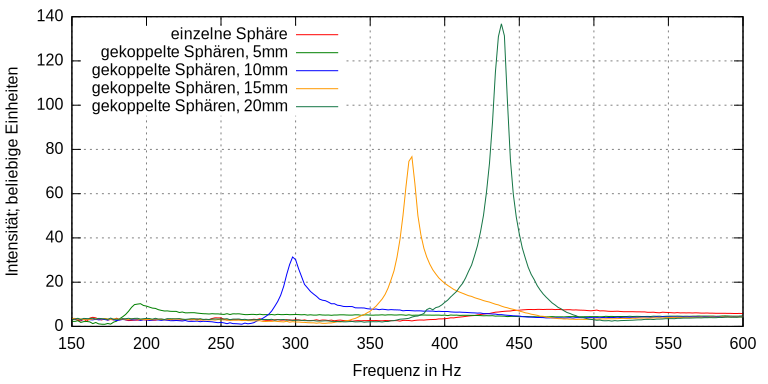
\includegraphics[width=\textwidth]{messwerte/doppelsphrenspektrum.pdf}
	\caption{Spektrum der gekoppelten Sphären bei Veränderung des Blendendurchmessers} \label{img:doppelspek}
\end{figure}

\begin{figure}[H]
	\centering
	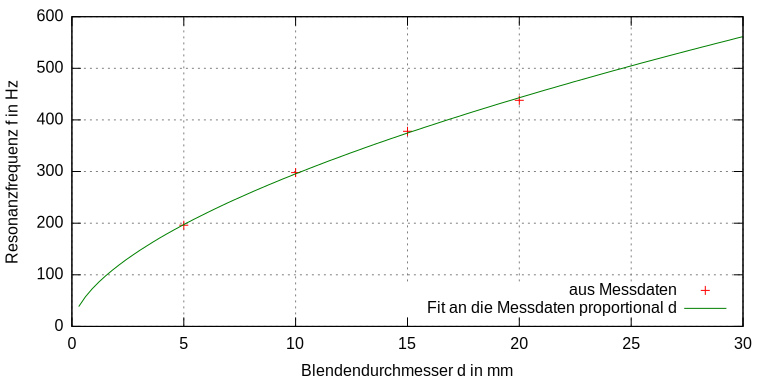
\includegraphics[width=\textwidth]{messwerte/resonanzendoppelsphre.pdf}
	\caption{Resonanzfrequenzen der Doppelsphäre in Abhängikeit vom Blendendurchmesser}\label{img:reskopp}
\end{figure}
\vspace{-2em}
\section{Quellen}
\begin{itemize}
	\item \url{https://de.wikipedia.org/wiki/Stehende_Welle}
	\item Vorlesung "`Quantenmechanik I"', gehalten von M. Schlanges im Sommersemester 2014
	\item \url{https://de.wikipedia.org/wiki/Wellengleichung}
	\item Versuchsanleitung "`Quantum Analogs"' und beinhaltete Quellen
\end{itemize}
\end{document}